\documentclass[authoryear]{elsarticle}
\usepackage{amsmath}
\usepackage{graphicx,psfrag,epsf,comment}
\usepackage{enumerate}
\usepackage{url} % not crucial - just used below for the URL 
\bibliographystyle{chicago}
\usepackage{threeparttable}

\newcommand{\logit}{\mathrm{logit}}
\newcommand{\I}{\mathrm{I}}
\newcommand{\E}{\mathrm{E}}
\newcommand{\p}{\mathrm{P}}
\newcommand{\e}{\mathrm{e}}
\renewcommand{\o}{\omega}
\newcommand{\vecm}{\mathrm{vec}}
\newcommand{\kp}{\otimes}
\newcommand{\diag}{\mathrm{diag}}
\newcommand{\cov}{\mathrm{cov}}
\newcommand{\eps}{\epsilon}
\newcommand{\ep}{\varepsilon}
\newcommand{\obdots}{\ddots}    % change this later
\newcommand{\Ex}{{\cal E}}
\newcommand{\Ax}{{\mathrm{A}}}
\newcommand{\Exd}{\Ex_d}
\newcommand{\Es}{\Ex}
\newcommand{\rat}{{\frac{c_{ij}}{c_{i,j-1}}}}
\newcommand{\rmu}{m}
\newcommand{\rsig}{  r}
\newcommand{\fd}{\mu}
\newcommand{\tr}{\mathrm{tr}}
\newcommand{\cor}{\mathrm{cor}}
\newcommand{\bx}[1]{\ensuremath{\overline{#1}|}}
\newcommand{\an}[1]{\ensuremath{a_{\bx{#1}}}}

\newcommand{\bi}{\begin{itemize}}
\newcommand{\ei}{\end{itemize}}

\renewcommand{\i}{\item}
\newcommand{\SR}{\ensuremath{\mathrm{SRISK}}}
\newcommand{\sr}{\ensuremath{\mathrm{srisk}}}
\newcommand{\br}{\ensuremath{\mathrm{base\ risk}}}
\newcommand{\st}{\ensuremath{\mathrm{strain}}}
\newcommand{\pr}{\ensuremath{\mathrm{strain}}}
\newcommand{\cs}{\ensuremath{\mathrm{CS}}}
\newcommand{\cri}{\ensuremath{\mathrm{Crisis}}}
\newcommand{\var}{\ensuremath{\mathrm{VaR}}}
\newcommand{\covar}{\ensuremath{\mathrm{CoVaR}}}
\newcommand{\med}{\ensuremath{\mathrm{m}}}
\newcommand{\de}{\mathrm{d}}
\renewcommand{\v}{\ensuremath{\mathrm{v}_q}}
\newcommand{\m}{\ensuremath{\mathrm{m}}}
\newcommand{\tvar}{\ensuremath{\mathrm{TVaR}}}
\renewcommand{\c}{\ensuremath{\mathrm{CoVaR_q}}}
\renewcommand{\v}{\ensuremath{\mathrm{VaR}_q}}

\newcommand{\eref}[1]{(\ref{#1})}
\newcommand{\fref}[1]{Figure \ref{#1}}
\newcommand{\sref}[1]{Section \ref{#1}}
\newcommand{\tref}[1]{Table \ref{#1}}
\newcommand{\aref}[1]{Appendix \ref{#1}}


\newcommand{\cq}{\ , \qquad}
\renewcommand{\P}{\mathrm{P}}
\newcommand{\Q}{\mathrm{Q}}

\newcommand{\Vx}{{\cal V}}

\newcommand{\be}[1]{\begin{equation}\label{#1}}
\newcommand{\ee}{\end{equation}}

\newcommand{\D}{\mathrm{D}}




\begin{document}

\title{An early warning system for monitoring  stress in the financial system}
%\author[acst]{Piet de Jong\corref{cor1}\footnote{The authors gratefully acknowledge CIFR, the Centre of International Financial Regulation for financial support and other assistance}}
%\ead{piet.dejong@mq.edu.au}
%\author[acst]{Geoffrey Loudon}
%\author[acst]{Weihao Choo}
%\address[acst]{Department of Applied Finance and Actuarial Studies Macquarie University, NSW 2109, Australia.}
%\cortext[cor1]{Corresponding author}


\begin{abstract}
SRISK methodology recently proposed in the literature is refined and extended using a formalised stress testing framework.  The framework distinguishes between two types of risk:  basis risk and stress risk.
basis risk is defined as 

 Both expectations are  based on a time series model and  observations to date.   Stressed expectation differs from the ordinary expectation in the imposition of an additional hypothetical  stress, modelled using a stress function and scenarios.  Stress risk is the difference between stressed expectation and ordinary expectation.  Stress functions are chosen by the practitioner and  exaggerate the probability undesirable  outcomes.    Properties and characterisations of stress and stress related quantities are displayed and explored.  Systemic stress is defined in terms of stresses   impacting groups of firms or financial entities.    Application is made to the study of the stability of Australian banks using daily time series data.
\end{abstract}

\date{}
\maketitle
\noindent
{\it Keywords:}  Capital shortfall, basis risk, stress testing,  stressed expectation, stress diversification.


\newpage

\section{Introduction}\label{intro}
Monitoring stresses and systemic risk in the financial system is a key function of macro--prudential regulation. Central banks and other financial regulatory bodies such as the US Financial Stability Oversight Council, the European Systemic Risk Board and the Australian Prudential Regulation Authority (APRA) are concerned with developing and applying early warning quantitative  measures  to warn of potential episodes of heightened systemic risk. 

Systemic risk has many dimensions. For example, in their influential review paper, \cite{Bisias2012} present a taxonomy of six categories of systemic risk comprising 31 quantitative risk measures. While attempts to gain consensus on a theoretical definition have proved elusive, several empirical measures of systemic risk have been developed and applied with  success.  An important example is the SRISK measure due to \cite{brownlees2015} -- an index that measures the expected capital shortfall of a financial institution conditional on a large and lengthy decline in equity markets. \cite{brownlees2015} show that their SRISK based measures are able to identify systemically important financial firms and are informative about the impact of financial crises on future macro-economic conditions. 

This paper refines and extends the SRISK model of \cite{brownlees2015} in  key ways. First SRISK is formalised  as a put on the expected shortfall with the ordinary expectation defined as the basis risk (\br) associated with the put.   Using a stress function  the so--called stressed expectation is used to measure the impact of stress.   Stressed expectation can be similar to the \cite{brownlees2015} conditional expectation given  a severe market downturn.  However our generalised methodology  permits a more flexible definition of stress and a wider class of ``stressors" including stress defined in terms of  a number of extreme outcomes.  The difference between the stressed and ordinary expectation is defined as the stress risk associated, called \pr\ where P stand for psi,  the function $\psi$ modelling the stress. 

\br\  and \pr\  capture different aspects of stress on a firm. \br\  is a function of existing volatility and leverage. As these factors increase, \br\  rises and this makes the firm more susceptible to \pr, regardless of the stress event itself.   Properties of \pr\  are explored.
   
\cite{brownlees2015} define stress by conditioning on an absolute cutoff of arbitrary size and length. With time dependent volatility or uncertainty, absolute cutoffs  are less meaningful and our development suggests  it is  useful to specify conditional behaviour in percentile terms relative to current market conditions. This yields a sharper focus on the incremental impact of further stress and permits a more incisive view of the  implications from SRISK numbers. These extensions provide additional insights into the sources and economic nature of for example systemic risk. The measures provide potentially new and improved ways of anticipating episodes of heightened systemic risk. Their practical use can be expected to help regulators monitor risk including systemic risk and contagion in timely fashion,   facilitating remedial action where necessary.

While our measures are designed for use in all financial systems, it is of particular interest to test them using the Australian setting for at least two reasons. First, the Australian financial system is dominated by only four banks. In Australia there are four major banks that hold 78\% of the total assets of all Authorised Deposit-taking Institutions in  Australia.\footnote{Based on balances at 31 December 2014 disclosed in APRA's Quarterly Authorised Deposit-taking Institution (ADI) Performance Report for March 2015.} It is therefore obvious that the four majors are systemically important and the remaining ADIs are not so unless stress in one of these minors somehow creates financial contagion to the majors, in an unforeseeable way. Second, the Australian banking system proved to be resilient through the recent global financial crisis (GFC), implying that systemic risk did not reach the extreme levels experienced by other countries where bank failures occurred. Both these features of the Australian system suggest that it may be difficult to find useful additional information about systemic risk by refining quantitative measures like SRISK. Since we are able to show that our measures are informative about systemic risk in Australia, we conjecture that they will provide additional insights elsewhere.  

The nature and usefulness of our measures are demonstrated using publicly available daily financial data for the eight Australian banks detailed in \tref{eightbanks} spanning the period from  3 April 2000 through to 1 December 2014.  The data is described in detail in \aref{data}.  Prices, adjusted for dividends are plotted in \fref{prices}.  Prices are combined with number of shares to derive total equity. Total debt for each firm is also collected from annual accounting reports. 

Remaining sections are structured as follows. Section \ref{litrev} briefly discusses related literature. Section \ref{capshort} defines current and future  capital shortfall similarly as \cite{brownlees2015} under a simple Basel II regulatory framework. The definition of systemic risk used by \cite{brownlees2015} is discussed, refined and improved in \sref{srisk}. Applications to Australian bank data are discussed in \sref{simulate} and \sref{simulate1}. Section \ref{aggregate}  discusses the aggregation of  stresses across firms with and without allowance for merging or diversification. Section \ref{monitoring} displays stress calculations as they would proceed in real time.   Section \ref{riskmethod} offers an alternative modelling approach, based on assets.  Section \ref{conclude} concludes.

\begin{table}[htbp]
\label{banks}\caption{Major and minor Australian banks}\label{eightbanks}
\begin{center}
\begin{tabular}{l|l|l|l}
\hline
 \multicolumn{2}{c|}{major}& \multicolumn{2}{c}{minor}\\
 \hline
CBA & Commonwealth Bank  & MQG & Macquarie \\
ANZ & Australia \& New Zealand  & BOQ & Bank of Queensland\\
NAB & National Australia  & BEN & Bendigo and Adelaide \\
WBC & Westpac & ABA& Auswide \\
\hline
\end{tabular}
\end{center}
\end{table}%


\begin{figure}[htbp]
\label{prices}
\begin{center}
 \begin{tabular}{cc}
      \resizebox{55mm}{!}{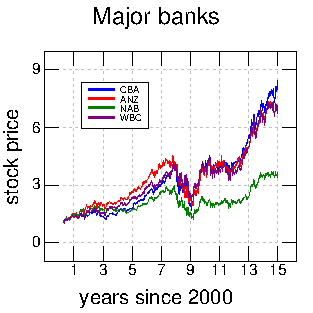
\includegraphics{figures/fig1a.pdf}} &
      \resizebox{55mm}{!}{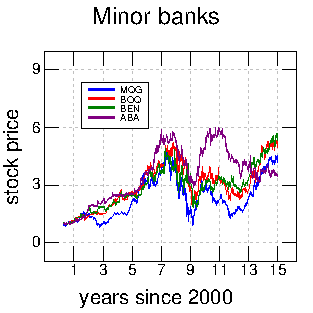
\includegraphics{figures/fig1b.pdf}}\\
    \end{tabular}
\caption{Daily stock  prices of four major (left panel) and four minor (right panel) Australian banks 2000--2014.  Price series normalised to start at 1.}
\end{center}
\end{figure}


\section{Literature review}\label{litrev}
Many papers in the finance and economics literature are devoted to the development and application of a variety of quantitative measures of systemic risk or financial stress. \cite{Bisias2012} provide an instructive and qualitative survey of numerous measures in use. \cite{Giglio2015} supply empirical evidence on the ability of many of these measures, both individually and collectively, to provide early warning signals of deterioration in macro-economic conditions. In this section, we provide a selective overview of those measures most closely related to SRISK and its relevance for assessing systemic risk in the financial sector. 

The genesis of SRISK lies in a series of papers including \cite{acharya2012aer}, \cite{acharya2012wp} and \cite{brownlees2010volatility}. In these papers, SRISK is defined as the expected capital shortfall of a financial firm, conditional on a crisis. A crisis is deemed to occur whenever a relevant market index suffers a significant decline over a chosen horizon. SRISK measures require an estimate of the long run marginal expected shortfall (LRMES) typically obtained by simulation methods.

\cite{brownlees2015}  develop empirical methodology to construct SRISK measures. SRISK depends on the firm's size, leverage and its LRMES. The LRMES is obtained by assuming a dynamic process for the joint distribution of firm and market returns. \cite{brownlees2015} use  the standard GARCH-DCC model of \cite{engle2002dynamic} with threshold ARCH volatilities on the basis that this represents a good trade-off between model complexity and prediction accuracy. The LRMES is computed as the Monte Carlo average of simulated multi-period returns,  conditional on the return being worse than the cut-off level chosen to identify a financial crisis. Using a sample of large US financial firms,  \cite{brownlees2015} show the practical usefulness of their measure in three ways: (i) SRISK rankings identify systemically risky US banks during the GFC; (ii) pre-crisis SRISK helps predict capital injections by the Fed Reserve; (iii) aggregate SRISK provides early warning of declines in industrial production and higher unemployment.
     
\cite{Engle2015} extend the model in \cite{brownlees2015} to incorporate global, country and industry effects. This extended model makes  use of the \citep{Engle2014dcb} dynamic conditional beta model. Their empirical methods are able to provide information about the relative systemic importance of industry type and country identity. For instance, they find  that systemic risk in Europe during the GFC was predominantly due to banks while France and the UK recorded the largest country-level SRISK numbers. 

\cite{adrian2011covar} propose an alternative measure of systemic risk  emphasising the co--dependence of financial firms and the importance of risk spillovers within the financial sector. They introduce CoVaR$_i$ which computes the Value--at--Risk (VaR) of the entire financial system, conditional on institution $i$ being in distress. Distress is defined as the state where the institution is exactly at its VaR level. \cite{Girardi2013} improve CoVaR by conditioning on the institution being at most at its VaR. This generalisation is useful as it takes into account the severity of tail losses and facilitates back--testing of CoVaR. 

\cite{acharya2012aer} relate SRISK and CoVaR and demonstrate that assuming the joint distribution of returns is conditionally normal, SRISK is a more complete measure. \cite{Benoit2013} show how several popular systemic risk measures including MES, CoVaR and SRISK are different transformations of market risk measures and derive those conditions under which they provide similar rankings of systemically important financial institutions.

Empirical estimates of SRISK  requires a model for the joint distribution of returns of individual firms and the market. Many of these papers use \cite{engle2002dynamic}'s GARCH--DCC model aiming to capture the time-varying dynamics of the return (co)variances in a feasible manner. While we also use this model in our empirical analysis, we emphasize that our approach can utilise any appropriate model for simulating the joint distribution of firm and market returns going forward. 

\section{Capital requirements, leverage and future shortfall}\label{capshort}

If $d$ and $w$ are the debt and equity, respectively, of a  firm  and $k$ is the prudential requirement,  then  following \cite{brownlees2015}, the   capital requirement is
\be{capreq}
k (d+w)-w = k d\left(1-\frac{1-k}{kL}\right)=kd\left(1-\e^{-\ell}\right)
\ ,
\ee
where
\be{lev}
L=\frac{d}{w}\cq \ell=\ln\left(\frac{kL}{1-k}\right) = \logit(k) + \ln(L) \ .
\ee
The capital requirement \eref{capreq} is positive if $\ell>0$. Note $kd$ is the proportion of debt $d$ required as capital if equity $w=0$.  Each unit of  $w$ is counted $1-k$ towards required capital.     Alternatively $k$ is the proportion of assets $d+w$ excluded from capital calculations, and higher $k$ leads to higher capital shortfall.   

A negative capital requirement -- that is a   surplus relative to requirements -- occurs  if $\ell<0$.   The default index $\ell$ is the rate of return $r$ that must be achieved in order for the firm to be on the just out of  default.   The default index $\ell$ depends on $k$, the prudential fraction. 

\subsection{Basel default}
If $k=8\%$ and  \eref{capreq} is positive then the  firm or financial institution is said be in ``Basel default" or a ``Basel breach" has occurred.  The value\footnote{See for example \cite{brownlees2015}.} $k=8\%$ is the Basel fraction and  implies $\logit( k)=-2.44$ and
$
\ell = \ln(L) - 2.44
$.   A firm is said to be in Basel default if the default index $\ell>0$ and $\ell$ can be considered as an index of the degree to which a firm is in default.  Note  $\logit(k)$ enters $\ell$ as an additive constant and has  minor role in the subsequent technical development and can be varied to test for sensitivity to $k$.  

The shorfall definition \eref{capreq} is simplistic and restrictive.   The definition and value $k=8\%$ is used here to conform to the previous literature and provide an easily accessible  platform to the key results of this paper,  without becoming entangled in precise and perhaps more realistic definitions of shortfall.   \sref{riskmethod} deals with a more realistic but more intricate definition.  

\fref{Bloglev} displays default index $\ell$ with $ k=8\%$ for the four major and four minor Australian banks listed in \tref{banks} on the first trading day of each month from January 2003  through to December 2014.  Note most banks are Basel compliant up to about 2008, entering into Basel default from 2009 as a result of the GFC. Prolonged Basel defaults are experienced for some banks, notably NAB.


\begin{figure}[htbp]
\begin{center}
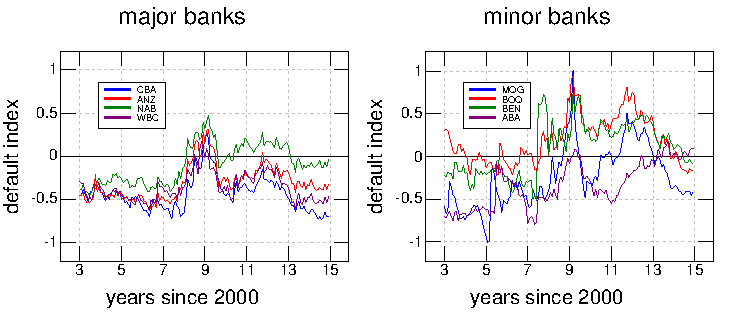
\includegraphics{figures/fig2.pdf}\caption{Basel default index  for four major (left panel) and four minor (right panel) Australian banks from the beginning of 2003 through to end of 2014.  All banks contravene the threshold (corresponding to the zero horizontal) around the start of 2009.}\label{Bloglev}
\end{center}
\end{figure}

\subsection{Future capital requirement and shortfall}

Financial institutions and regulators are concerned with future capital requirements, say in in a months time and in particular any potential shortfall.   Given the definition \eref{capreq}  the future capital requirement of the firm depends on the future return on equity $r$.   The future future equity is then  $w\e^{r}$ and assuming, as in \cite{brownlees2015} debt $d$ is constant, the  future capital requirement is, per unit $kd$ and analogous to \eref{capreq}, 
\be{fcapreq}
   S=1-\frac{1-k}{kL\e^{-r}} =1-\e^{r-\ell}\ .
\ee
The future return $r_i$ is unknown but its probability distribution may be relatively well understood and modelled.  Note $-\infty<S\le 1$ with $S=1$ indicating the future capital requirement is $kd$.

The positive part of \eref{fcapreq} is the future capital shortfall per unit $kd$
\be{bs}
S^+ = \left\{\begin{array}{lr} 0\ , & r\ge \ell\ ,\\ 1-\e^{r-\ell}\ , & r<\ell\ ,\end{array}\right.  
\ee
where $^+$ denotes the ``positive part of."  
Thus $S^+$ is  a put\footnote{Since $\E(S^+)=\E(S>0)\E(S|S>0)$ where   $\E(S^+)$ is the default probability  and $\E(S|S>0)$ is a measure of ``tail risk."   Both the default probability and tail risk are  defined relative to  $k$.  Since the expectation is ``normal" the probability and tail risk are both ``base" cases.} on the return $\e^{r-\ell}$ with strike 1 and $0\le S^+\le 1$.  From \eref{bs}, the  default index $\ell$ is the rate of return $r$ that must be achieved over the future period for the firm to just attain Basel solvency.   Default put options similar to \eref{bs} have been discussed in the insurance literature as critical to an evaluation of a firm:  see for
example \citet{merton1977analytic}, \citet{doherty1986price}, \citet{cummins1988risk}, \citet{myers2001capital} and \citet{sherris2006solvency}.



\subsection{Projecting future shortfall -- motivating example}
In subsequent sections  time series methods are used to project future capital requirements \eref{fcapreq}  and in particular future shortfall $S$ defined in \eref{bs} for different firms $i$, under basis conditions and under stressed scenarios.   These forecasts are used to determine the stress of both individual firms $i$ and the system as a whole.   To understand the basis of the approach \fref{simulation},   displays two snapshot outputs from projections generated as described  in \aref{garchdcc}:  6000  simulated one month ahead projected returns for  CBA and the wider market, on  two dates: the first trading day in January 2009 and the first trading day in December 2014.  The CBA returns are used to calculate the future shortfall per units $kd$ as in \eref{fcapreq}.  Both panels use the same horizontal and vertical scales.   Based on the available data at those two points in  time, policy makers and regulators faced entirely different projections.   The scatter of dots are the forward simulations.  Note there is no hindsight bias as the model at each time point is based on the available data to that point in time.     In the left panel $S>0$ and a positive capital shortfall is projected for most scenarios.    In the right panel $S=0$ and the banks are projected to have capital surpluses relative to requirements for any conceivable market scenarios.

 The black dots in each panel indicate the actual outcome after one month.    In the left panel the outcome is a decline in both  the market and CBA stock price.    In the right panel there is slight decline in the stock price, and a more substantial market downturn.    Thus at the beginning of January  2009 the one month forward projection for  CBA was far from compliance, while in December 2014 the one month forward projection is of complete compliance.

The two panels  display very different volatility and slopes. In January 2009 both CBA and the market return distributions are highly volatile and correlated. The correlation remains strong in December 2014 but with less return volatility.  Subsequent sections of this paper use time series of these  snapshots  to compute cross sectional and longitudinal basis and systemic stresses.

\begin{figure}[htbp]
\begin{center}
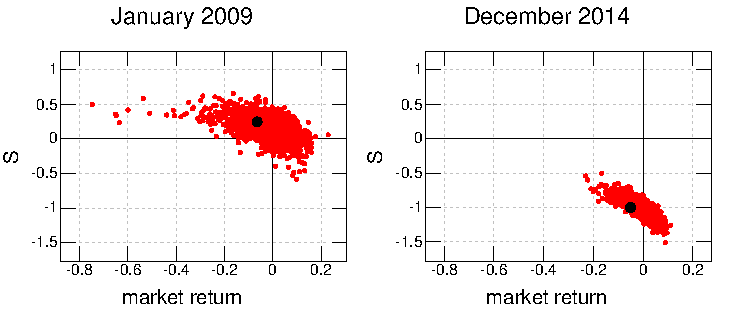
\includegraphics[width=12cm]{figures/figCBA.pdf}
\caption{Forecast bivariate distribution of $C$ the projected  one month ahead capital requirement for CBA per unit $kd$ versus the market rate of return at start of January 2009 (left panel)  and December 2014 (right panel). Note scales in both panels are the same, the relatively large volatility in the left panel, and the left skew in the  marginal distributions.  Black dots indicate actual  outcome at the end of each month.}\label{simulation}
\end{center}
\end{figure}

\section{Monitoring systemic risk}\label{srisk}

 \cite{brownlees2015} define  systemic risk\footnote{In contrast to \cite{brownlees2015} we factor out the scale factor $kd$ making for a more transparent 0 to 1 scale for \SR.} for a group of firms in terms of the expected future capital requirement $S_i$ for each firm $i$ in the group:
\be{esrisk}
\SR =  \sum_i \pi_i\left\{\Es(S_i)\right\}^+ = \D[\{\Ex(S_i)\}^+]\cq \pi_i = \frac{d_i}{d}\cq d=\sum_id_i \ ,
\ee
where $S_i$ is the shortfall \eref{fcapreq} for firm $i$.
Here $\Es$ denotes expectation given the systemic event of a major general market downturn and $\D$ is debt weighted averaging.    Further \SR\ is expressed in units $kd$ and $0\le\SR\le 1$ with \SR\ near 1 indicating extreme financial distress for all firms. \SR\ is based on the expected capital requirement and firms with an expected capital surplus under stress are ignored.   The expression \eref{esrisk} slightly modifies the definition  of \cite{brownlees2015} by dividing their \SR\ expression by $kd$. 

The proportional contribution of firm $i$ to \SR \eref{esrisk}  is defined by   \citep{brownlees2015} as
\be{sriskperc}
\SR_i=\frac{\pi_i\{\Ex(S_i)\}^+}{\SR} \ .
 \ee
 Note $0\le \SR_i\le 1$ with larger values indicating firm $i$ is systemically important: it holds a high proportion $\pi_i$ of the total debt, and/or is likely to heavily breach the Basel capital requirement.  Expression \eref{sriskperc} depends on $k$ through each of the default indexs $\ell_i$. 

In this article we propose four modifications to \SR\ and $\SR_i$ defined in \eref{esrisk} and \eref{sriskperc}.   These modifications are designed to improve stress monitoring.  The  modifications  are shown,  theoretically and empirically, to have more  sensitivity and specificity.   Sensitive, in the sense of more likely detect  firms likely to face financial distress.   Specific in the sense of   minimising false alarms.  The modifications are:
\begin{enumerate}
\item  Replacing $\{\Es(S_i)\} ^+$ in \eref{esrisk} and \eref{sriskperc} by $\Es(S_i^+)\ge\{\Es(S_i)\} ^+$. The justification is that typically $\Es(S_i)=0$ and  hence \eref{esrisk} is not affected by firms that  have zero expected capital requirement even though in individual instances that capital requirement may be large.   Using $\Ex(S^+_i)$ instead of $\Ex(S_i)$ implies each firm counts with degree depending on the its proportionate contribution $\pi_i$ to total debt and the expected value of a put on its shortfall.  Thus the analogue of \SR\  in \eref{srisk} is 
\be{srisk2}
\sr=\Ex\{\D(S_i^+)\} = \D\{\Ex(S_i^+)\} = \sum_i\pi_i(\sr_i)\ ,
\ee
where $0\le \sr_i\le 1$ and $\pi_i(\sr_i)$ is the proportion of \sr\ originating in firm $i$.
 
\item Using more general   definitions of $\Es$ to encompass more flexible stress specifications.   Modelling stress  as  10\% market general market downturn or more, while interesting, is obviously arbitrary.   This paper posits more flexible and robust specification of stressed expectation $\Ex$.   This is discussed in \sref{formal}.

\item The srisk defined in \eref{srisk2} is broken up into two components
\be{breakup}
\sr=\D\{\E(S_i^+)\}+\D[\{\Ex(S_i^+)\}-\E(S_i^+)\}]\ . 
\ee
called the base risk and strain, respectively.     Hence \sr\ is a debt weighted average of base risks and strains.       A firm counts highly in \sr\  if it carries a significant portion of total debt,  has high base risk and  high strain.  

\item Pooled base risk is defined as  $0\le\E(S^+)\le 1$ where $S=\D(S_i)$.  Similarly pooled strain is  
$\Ex(S^+)-\E(S^+)$.  

\item Non--pooled shortfall is defined as $S^*=\sum_iS_i^+$ with non--pooled base risk $\E(S^*)$ and strain $\Ex(S^*)-\E(S^*)$.  

\item Similar to before, $\Ex(S_i^+)=\Ex(S_i^+>0)\Ex(S_i|S_i>0)$.   The two factors on the right are called the stressed default probability and stressed tail risk, respectively.    The measures
$$
\Ex(S_i^+>0)-\E(S_i^+>0)\cq \Ex(S_i|S_i>0)-\E(S_i|S_i>0)
$$
are the default probability and tail risk strain, respectively. 

\item    System  base resilience  is measured with the positive number 
\be{resil}
 \ln \frac{\E(S^*)}{\E(S^+)} = \ln\frac{\E(S^*>0)}{\E(S^+>0)} + \ln\frac{\E(S^*|S^*>0)}{\E(S^+|S^+>0)}\ .
\ee
A large value indicates shortfall in individual firms can be absorbed in the system.   A value near zero indicates there is no capacity for the system to absorb shortfall in individual firms.  Using $\Ex$ instead of $\E$ in \eref{resil} yields the resilience under stress.
 
\end{enumerate}
 

\section{A formal framework for systemic risk measurement}\label{formal}
The  proposed improved framework considers future capital shortfall $S$ as defined in \eref{fcapreq}  for a a single firm or group of firms.   Then the framework for measuring stress may focus on $S$, the positive part  $S^+$ as defined in \eref{bs}, or a more general function of $S$.   For concreteness suppose the focus is on $S^+$.

The improved framework consists of:
\bi
\i  A collection of scenarios generically labelled $\omega$ where  $\omega$ discrete or continuous.  Scenarios may be both benign or serious in terms of their potential impact on shortfall $S$.   Scenarios $\omega$ are systemic if they have potential impact on many firms.  

\i The ``natural" probability of scenario $\omega$ is $p(\omega)$.   If $\omega$ is continuous then $p(\omega)$ is interpreted as a probability density.

\i  Basis strain is defined as the ordinary expectation
$$
 \E(S^+)=\sum_\omega p(\omega) \E(S^+|\omega)\cq 0\le\E(S^+)\le 1\ .
$$
For continuous $\omega$,  the sum is interpreted as an integral. 


\i  A stress function $\psi(\omega)\ge 0$ defined on the  scenarios $\omega$ with  $\E(\psi)=1$.  The stress function serves to amplify or downplay the importance of different scenarios.   On average the amplification is 1.   The stress function serves to ``bias" outcomes towards ``stressful" scenarios, that is scenarios likely to drive up shortfall.
  
\i The \sr\ of a firm is the expected shortfall under the stressed probabilities $\psi(\omega)p(\omega)$:
\be{formula}
\Es(S^+) = \E\{\psi\E(S^+|\psi)\}=\E(\psi S^+)=\E(S^+)+\cov(S^+,\psi)\ ,
\ee
where the last equality follows since $\E(\psi)=1$.   Note $0\le\Ex(S^+)\le 1$.     
The import of $\psi(\omega)$ is to change the natural probabilities $p(\omega)$ to ``stressed" probabilities $\psi(\omega)p(\omega)$.   

 \i The strain is defined as the additional expectation due to stress 
 $$
\Es(S^+)-\E(S^+)\cq \mathrm{srisk} = (\mathrm{base\ risk})+\mathrm{strain}\ \ .
 $$

 
 \i Note that 
 $$
 \ln\frac{\Ex(S^+)}{\E(S^+)} = \ln \frac{\Ex(S>0)}{\E(S>0)} +\ln\frac{\Ex(S|S>0)}{\E(S|S>0)}\ .
 $$
 That is, the approximate percentage change in risk due to stress is the the percentage change in the default probability plus the percentage change in the tail risk.
  \ei




\subsection{Practical stress functions}
The simplest example is where $\psi(\omega)=0$ except for a single  scenario $\omega$ where it is equal to $1/p(\omega)$.   In this case all probability is transferred to the single scenario $\omega$ and $\Es(S)=\E(S|\omega)$.  
This conditional expectation is often modelled and computed with a spreadsheet.

The stress function used in  \cite{brownlees2015} is where $\omega$ is the market return and $\psi(\omega)=0$ unless $\omega\le 0.1$ in which case $\psi(\omega) = c$ where $c$ is 	 such that the area under $\psi$ is 1.   In other words scenarios are different market returns with stress being zero unless market return is  a drop of 10\% or more.   This stress function is quite blunt:   stress is either on or off and if on there is no reckoning as to the degree of stress.

A richer example is where $\omega$ is the percentile of a variable such as the overall market return, measured relative to the current  market return distribution.   Then $p(\omega)$ is the uniform density on the unit interval.   If 
$$
\psi(\omega)=n\{1-(1-\omega)^{n-1}\}\ ,
$$
then $\psi$ is the density of the worst percentile outcome in $n$ independent trials.   In this case \pr\  corresponds to the increase in risk when the general market has its worst outcome in $n$ independent trials given the current return distribution.  This stress function  is used to study stress in Australian banks in \sref{simulate1}.  If $n=1$ then $\psi(\omega)=1$, there is no stress, and $\Es(S)=\E(S)$ and \pr=0.

Another example, close to that implemented in \cite{brownlees2015} is where $\omega$ is a percentile with $\psi(\omega)=1/c$ for $\omega<c$ and 0 otherwise.   In this case  $\Es(S)=\E(S|\psi<c)$ and \pr\  is the difference between the   tail and ordinary expectation.
More general stressed expectations of the form of \eref{formula} are discussed in \cite{furman2008weighted1} and \cite{choo2010determining}.

\subsection{Strain potential} 

A  measure of potential for a stress function $\psi$ to induce strain is its volatility denoted $\sigma_\psi$. If $\psi$ is constant then $\sigma_\psi=0$.   If $\psi(\omega)$ picks out a single scenario $\omega$ then 
$$
\sigma_\psi= \e^{-\logit\{p(\omega)\}/2}\ ,
$$
which is large if the scenario probability $p(\omega)$ is small. 

Standardised strain is: 
$$
\beta_\psi= \frac{\mathrm{strain}}{\sigma_\psi}=\sigma_{S^+} \times\cor(S^+,\psi)\ .
$$
measuring the departure of $\Es(S)$ from $\E(S)$ in units of $\psi$ volatility. Here $\cor$ denotes correlation. The measure $\beta_\psi$ facilitates the comparison of strain on $S$ across different stressors and has the interpretation of a regression coefficient:
$$
\E(S^+|\psi=x) \approx (\br) +\left(\frac{\st}{\sigma_\psi}\right)\left(\frac{x-1}{\sigma_\psi}\right)\ .
$$
Thus $\beta_\psi$ measures, in minimum mean square error sense, the change in strain as stress increases by one standardised unit.

 Strain can also be measured  in units of $S$ volatility:
$$
\frac{\Es(S^+)-\E(S^+)}{\sigma_{S^+}}=\sigma_\psi\cor(S^+,\psi)\ .
$$
This measure gauges the extremity of strain.

\subsection{Computing basis strain and stress strain via simulation}
Given $N$ simulations $\omega\sim p(\omega)$ and $S(\omega)\sim p(S|\omega)$  then  $S(\omega)\sim p(S)$ and  
$$
 \frac{1}{N}\sum_\omega S^+(\omega)\rightarrow \E(S^+) \cq \frac{1}{N}\sum_\omega \psi(\omega)S^+(\omega)\rightarrow \Ex(S^+) \ ,
$$
as the simulation effort $N$ increases.

If $\psi$ is based  on percentile outcomes   then the simulated $\omega$ are ranked and $\psi(\omega)$ is computed from the empirical rank of $\omega$.  If $\omega$ has many components corresponding to percentiles of different variables then $\psi(\omega)$ is a copula density chosen to induce appropriate  tail dependence.

 As in \cite{brownlees2015},  $\omega$ in the next section is the projected  market return while $S(\omega)$ or more particularly $S_i(\omega)$  is the shortfall for firm $i$ based on its projected rate of return $r_i$ given the market return $\omega$.   The joint distribution of $\omega$ and $r_i$ is simulated  from  fitted bivariate time series models.  The market return is used as the stressor with the stress function $\psi$ modelling  stress scenarios.

The time series models used are stochastic volatility models based on the GARCH--DCC framework of \cite{engle2002dynamic} summarised in \aref{garchdcc}. The GARCH-DCC model captures prolonged periods of high volatility and correlation in firm and market returns, typical in financial markets. The GARCH--DCC framework is one possible implementation.   For example future return scenarios may be constructed in a more ad--hoc manner e.g. judiciously constructed scenarios by regulators or policymakers.   The  framework set out in \sref{srisk} can be based on  any  generated  future  scenarios.

\fref{simulation} displays simulations from a joint distribution generated from the GARCH--DCC model estimated from daily returns.  The left panel utilises  one month forward simulated returns at the start of January 2008.   The market returns are on the x--axis while the shortfall $S$ corresponding to associated CBA return are on the y--axis.  Low market returns are likely to lead to sharply higher CBA shortfall, as compared to the right panel showing the same as at December 2014.   This is suggested by the slope of the scatter plots:  the left slope appears steeper than the right. This implies higher systemic stress in December 2008. In addition $S$ volatilities are much higher in the left panel compared to the right, indicating higher basis stress in December 2008. Also note that with a stressor function $\psi$ defined in terms of market return percentiles, the magnitude of a market downturn at a fixed percentile threshold is more significant in the left panel.

\section{Australian bank stress forecasts}\label{simulate1}

\fref{fig4} displays, in the top panels, the estimated basis risk for each major (left) and minor (right) Australian banks based on the projected one month ahead return distribution fitted using the GARCH--DCC model.  Note the return distributions are constructed from data only available at that time and hence are not affected by look--ahead bias.  The first inclinations of increasing basis risk occurs with NAB in early 2008 followed one month later by ANZ, and  a further few months later by WBC and CBA. basis risk subsided shortly after 2009, however basis risk for NAB rose again in 2011 and this sustained till 2013.  In general smaller banks are subject to higher basis risk after normalising for debt levels.


Bottom panels in \fref{default} show \pr\ computed by assuming the worst market return in 12 identical months. \pr\ for each bank generally exhibits similar patterns as \br. However, importantly, some banks have differing patterns which is an important observation for the regulator since \pr\ indicates sensitivity to market-wide downturns. For example ANZ had similar \pr\ stress as NAB around 2012 but lower \br. Hence although ANZ was not obviously in stress during 2012, it would be if a market downturn occurred. Bendigo and BOQ had high \br\ levels after 2008, but are overtaken by Macquarie in terms of \pr: Macquarie is more likely to suffer in a market downturn whereas Bendigo and BOQ are less likely to be impacted.

\begin{figure}[htbp]
\begin{center}
\includegraphics[width=12cm]{figures/fig4.pdf}
\caption{Basis strain  (top panels) and stress strain (bottom panels) based on one month ahead  forecasts $S_i^+$ for   major (left panel) and  minor (right panel)  Australian banks 2003--2014.  Stress is based on worst monthly market outcome in 1 year.  Note different y--scale on top and bottom panels.}\label{fig4}
\end{center}
\end{figure}

\fref{fig5} gives a picture of the relative magnitudes of \br\ and \pr\ in each of the eight banks.   For the major banks NAB stand out as, having \br\ more dominant than \pr\ and generally having heightened levels of \br.   ANZ appears to have relatively higher levels of \pr.    For the minors, MQG has persistently higher levels of \pr\ with BOQ and BEN comparable ratios and ABA having virtually no \pr\ compared to \br\ at any level of the latter. 

\begin{figure}[htbp]
\begin{center}
\includegraphics[width=12cm]{figures/fig5.pdf}
\caption{Historical relationship between stress strain and basis strain    for major   and  minor banks.}
\label{fig5}
\end{center}
\end{figure}


\section{Monitoring aggregate  stress and contagion}\label{aggregate}

This section uses two measures of future aggregate shortfall for a group of firms based on two different methods of aggregating default risk across firms:
$$
S^+ = \{\D(S_i)\}^+\le \D(S_i^+) =S^*\ .
$$
Here $S^+$ is referred to as the ``pooled" or ``diversified" shortfall with shortfall in one firm able to be offset by surplus elsewhere.  The shortfall $S^*$ is ``non--diversified" with shortfall in each firm $i$ adding up.

With $\Ex(S^+)$ heightened risk only arises if there is an ``on average"  shortfall.   Thus SRISK is relatively insensitive to tail events.  The second aggregation of risk displayed in \tref{dsrisk} uses $S^*$, the  sum of positive shortfalls across firms.  With $S^*$, shortfall within a firm is not offset by averaging  nor with surpluses in other firms. The measure is thus more sensitive to tail risk.
  
The second aggregation of risk displayed in \tref{dsrisk} uses $S^*$, the  sum of positive shortfalls across firms.  With $S^*$, shortfall within a firm is not offset by averaging  nor with surpluses in other firms. The measure is thus more sensitive to tail risk.

Our measures of basis and stress contagion are 
\be{cont}
\frac{\E(S^+)}{\E(S^*)}\cq  \frac{\Ex(S^+)}{\Ex(S^*)}- \frac{\E(S^+)}{\E(S^*)}
\ee
 both of which lies between 0 and 1.   A value near one indicates little of the risk in the group of firms, due to basis events or stress is absorbable and hence defaults are not diversifiable.   A value near 0 indicates virtually all of the risk in the system can ``diversified away." 
 
 \tref{dsrisk} displays and compares and contrasts the different definitions of risk. The last line of \tref{dsrisk} reproduces the \SR\  measure of \cite{brownlees2015}. Note $\Es(S)$ combines both basis stress, due to high volatility or leverage, and the imposed hypothetical stress. To understand the nature of stress it is important to understand the mix of these two different stresses.
 
 
\begin{table}[htbp]
\caption{Different strains}\label{dsrisk}
\begin{center}
\begin{tabular}{l|c|c|c}
\hline
& basis & strain & srisk\\
\hline
pooled &$\E(S^+)$ &$ \Ex(S^+)-\E(S^+)$ & $\Ex(S^+)$\\
non--pooled & $\E(S^*)$& $\Ex(S^*)-\E(S^*)$&$\Ex(S^*)$\\
\hline
resilience & $\ln\frac{\E(S^*)}{\E(S^+)}$& $\ln\frac{\Ex(S^*)}{\Ex(S^+)}-\ln\frac{\E(S^*)}{\E(S^+)}$&$\ln\frac{\Ex(S^*)}{\Ex(S^+)}$ \\
\hline
\SR & \multicolumn{2}{c}{$\D[\{\Ex(S_i)\}^+]$}\\
\hline
\end{tabular}
\end{center}
\label{default}
\end{table}%

System resilience aims to answer the question of whether the system as a whole can absorb shocks.   The capacity to absorb relies on implicit merging and hence on a measure of shortfall such as $S^+$.    When two firms merge the leverage of the resulting firm is less than that of the more highly leveraged firm.   The merged firm is more able to withstand return on equity shocks  unless negative shocks are more prone for the merged firm.   Similarly when many firms merge  puts $S^+$ for the conglomerate become less valuable.

Firms do not necessarily merge, even in dire financial circumstances.   Hence the mergers spoken of here are hypothetical.   From a regulators perspective, what would happen under a merger of all firms (or perhaps a group of firms) is nevertheless of interest.   A system as as a whole near Basel breach is more threatening that one where a few firms are near Basel breach but the system as a whole is strongly Basel compliant.

\section{Monitoring individual banks contribution to stress}

The proportionate contributions of bank $i$ to base risk, strain and \sr\ are 
\be{contrib}
\frac{\pi_i\E(S_i^+)}{\D\{\E(S_i^+)\}}\cq \frac{\pi_i\{\Ex(S_i^+)-\E(S_i^+)\}}{\D\{\Ex(S_i^+)-\E(S_i^+)\}}\cq \frac{\pi_i\Ex(S_i^+)}{\D\{\Ex(S_i^+)\}}\ ,
\ee
respectively. 

\begin{figure}[htbp]
\begin{center}
\includegraphics[width=12cm]{figures/fig6.pdf}
\caption{Projected one month  Australian banks risks through the financial crisis years 2008 through to the end of 2010.  Top panels are basis risk and stress risk.  Bottom left panel computes  basis and stress risk using pooling and no--pooling, and compares the same to \SR.   Bottom right panel displays contagion risk as defined in equation \eref{cont}.}
\label{fig6}
\end{center}
\end{figure}






\subsection{Aggregate stress in the Australian banking sector}\label{monitoring}
 \tref{jan2009} contains real time stress calculations on the first trading day of  January 2009.  As before there is no look ahead bias -- calculations on each of the two dates use data available on the first day of the applicable month.   The first eight rows in in the body of \tref{jan2009} correspond to the eight banks used in this study.  The first  and second columns in the two halves of the table body contain the default index  and debt  (as a percentage of total system debt) for each of the banks. 


The absorbance capacity is a measure of the system to absorb base risk, strain or srisk through merger.   If, for example, $\E(S^+)$ is much smaller than $\E(S^*)$ then a large portion of base risk can be ``diversified away" by merging firms.   This suggest the measures
$$
1-\frac{\E(S^+)}{\E(S^*)}\approx\ln\frac{\E(S^*)}{\E(S^+)}\cq \frac{\Ex(S^*)-\E(S^*)}{\Ex(S^+)-\E(S^+)}\cq \frac{\Ex(S^*)}{\Ex(S^+)} \ .
$$
The first and last measures lie between 0 and 1 with values near 0 
 near 0 indicating there is no pooling buffer. \tref{jan2009} displays the calculations for January 2009.

\begin{table}[ht]
 \caption{Analysis of bank  risk:  January 2009}\label{jan2009}
\centering
\begin{tabular}{l|rr|rrr}
 \hline
 & default & debt & \multicolumn{3}{c}{\% of non--pooled}  \\ 
 \cline{4-6}
bank & index  & \% & base risk & strain & $\mathrm{srisk}$\\
\hline
CBA & 18.57 & 24.30 & 22.99 & 29.60 & 25.20 \\ 
  ANZ & 15.93 & 18.37 & 14.87 & 18.89 & 16.21 \\ 
  NAB & 31.97 & 25.50 & 39.98 & 19.41 & 33.10 \\ 
  WBC & -1.55 & 22.84 & 5.86 & 23.94 & 11.91 \\ 
  MQG & 41.22 & 5.75 & 11.02 & 5.46 & 9.16 \\ 
  BOQ & 63.30 & 1.32 & 3.55 & 0.99 & 2.70 \\ 
  BEN & 18.91 & 1.81 & 1.72 & 1.71 & 1.72 \\ 
  ABA & -8.12 & 0.10 & 0.00 & 0.00 & 0.00 \\ 
  \hline
  \multicolumn{3}{r|}{non--pooled}  & 17.17 & 8.63 & 25.80 \\ 
  \multicolumn{3}{r|}{pooled} & 15.28 & 10.18 & 25.46 \\ 
  \multicolumn{3}{r|}{resilience} & 11.66 & -16.48 & 1.34 \\ 
   \hline
\end{tabular}
\end{table}

January 2009 was a time of great strain for all eight banks.       Six of the eight banks were in Basel default with positive capital shortfalls as indicated by the default index column:   the two banks not in Basel default were WBC and ABA.    
 
 Percentage base risk, strain and srisk    are displayed in the next 3 columns.    Most of the base risk arises from NAB -- almost 40\% of the total.   The next most base risk arises from  is CBA.   MQG  contributes almost double to base risk compared to the proportion of total debt  it carries.  The other three small banks contribute relatively little to base risk with BOQ  almost 3 times expected on the basis of its debt.   
 
Strain  is highest for the CBA, higher than expected on the basis of its debt load and hence CBA was most susceptible to stress from additional general market equity devaluation.    All other banks appear have strain comparable to their size in terms of debt load with only NAB having proportionally less strain.    This should be compared to NAB's high base risk.

The final two rows of \tref{jan2009} indicate the total amount of stress in the system and it's diversifiability.    
The second last  row labelled ``Total"  displays, in order, debt weighted default index, total \br\  and total \pr.  On aggregate Total \br\  is about twice \pr.   Thus there is more danger of increasing capital shortfall due to market volatility  as opposed to further stress from further substantial general market devaluation.  The final row indicates stresses are not diversifiable:    The marginally  smaller  ``diversified"  basis stress is offset by an increase in \pr.   

Stress readings  change dramatically when moving to December 2014 -- there is virtually no stress in any bank and the small amount of  stress in the system is diversifiable.    Most  \br\ is carried by NAB with lesser contributions by BEN and ABA.    All the stress in the minor bank ABA is basis stress as only NAB and NAB have substantial \pr\  contributions.   Again, however, it must be emphasised that there is minimal systemic stress in the system.  Notice total debt in the banking sector  jumps about 35\% between the two dates.

The two  panels of \fref{fig6} track  \br\ and \pr\ for the banking sector as a whole through time.   There is virtually no risk in the system till late 2007 and the early warnings show a buildup in \br\ in $S^*$ compared to $S^+$.   Thus initially all \br\ is diversifiable suggesting \br\ is building up in a few banks.   This pattern of diversifiability in \br\ is generally maintained except at the peak of the crisis at the beginning of 2009 and in late 2011.  This pattern of \br\ buildup is evident in the bottom panel displaying all \br\ is, for small levels of risk initially absorbable -- that is present in $S^*$ but not present in $S^+$. 

The top right panel in \fref{fig6} displays the time series behaviour of \pr.  Generally \pr\ is less than \br.   Further, in situations of elevated risk,  \pr\ in $S^+$ exceeds that in $S^*$ indicating systemic stress from a general market downturn is greater in the system as a whole than its constituent parts.   Again, however, as displayed in the bottom right panel, \pr\ initially builds up in $S^*$, and only later manifests itself in $S^+$.  However the buildup is rapid so that with significant \pr\ the level in $S^+$ exceeds that in $S^*$.



\section{Risk weighted asset methodology}\label{riskmethod}

The current stress framework can be used in conjunction with   the  risk weighting asset (RWA) methodology often used in determining capital shortfall.   RWA in effect assesses future stressed assets,   as opposed to, with SRISK,  future equity.   The same stress methodology can be used to stress assets.

Given debt $d$ and equity $w$ for a firm,  assets are
$$
d+w=\sum_ja_j\ ,
$$
where $a_j$ denotes the value of assets in asset class $j$.   Future shortfall is, equivalent to \eref{fcapreq},  
\be{shortfall2}
S=  d-(1-k)\sum_ja_j\e^{r_j}\ ,
\ee
where $r_j$ is the (uncertain) log--return on assets $a_j$.  With the risk weighting methodology the weights $a_j$  are replaced by $a_j/\sigma_j$ where $\sigma_j\ge 1$ is a ``risk" weight with large  weights assigned to  assets  with large perceived ``riskiness." 

Suppose $S$, $d$ and $r$ are the vectors of shortfalls, debts  and returns, respectively for the firms, and matrix $A$ has rows corresponding to the asset values of different firms.  Then the vector of firm shortfalls is
$$
S = d-(1-k)A\e^{r}\ ,
$$ 
where  exponentiation is componentwise.   Writing $S^+$ as the vector of positive shortfalls then, as in \sref{aggregate}, two aggregate measures of expected shortfall are $S^*= \sum_iS_i^+$ and $S^+=(\sum_iS_i)^+$ where $S_i$ is component $i$ of vector $S$.

Estimation of \br\ and \pr\ can proceed via simulation:
$$
\omega\sim p(\omega)\cq r(\omega)\sim p(r|\omega)
$$
where $r(\omega)$ is  the simulated vector of returns for the asset classes given scenario $\omega$.   The vector of shortfalls corresponding to $\omega$ is then $S(\omega)=d-(1-k) A\e^{r(\omega)}$  where $A$ is the matrix with row $i$ corresponding to the current asset values for firm $i$ and $\e^{r(\omega)}$ denotes componentwise exponentiation.   Then the vectors of \br\ and \pr, with components corresponding to the different firms $i$ are estimated as  
\be{srisk4}
\br\approx \frac{1}{N}\sum_\omega S^+(\omega)\cq
 \pr\approx \frac{1}{N}\sum_\omega  \{\psi(\omega)-1\}S^+(\omega)\ ,
\ee
with similar results for $S^*=\sum_iS_i^+$ and $(\sum_iS_i)^+$.  

Stressful scenarios can be implicitly constructed via the following percentile method.   Suppose $r\sim p(r)$ are simulations from the joint distribution of future asset returns.   Returns for each asset class are  ranked yielding simulated percentile vectors $\omega$.   Denote $S(\omega)$ as the vector of shortfalls computed as before from returns $r$ corresponding to $\omega$.   Then use these $S(\omega)$  in the expressions \eref{srisk4} with
$$
\psi(\omega) = nc(\omega)\prod_j \{1-(1-\omega_j)^{n-1}\}\ ,
$$
where $c(\omega)$ is a copula density designed to exaggerate the juxtaposition of  adverse percentile occurrences: such as exaggerated lower tail dependence.   If $c(\omega)= 1$  there is no exaggeration  and the copula associated with the $r(\omega)$ is the copula induced by $p(r)$.  If $n=1$ there is no sculpting of the marginal distributions.



\section{Conclusion}\label{conclude}

This paper presents a consistent methodology for stress testing and the measurement of  risk using the concept of stressed expectations.   Stressed expectation  formalises stress testing widely used in practice.  Stresses are introduced using a stress function and systemic stress uses a stress function based on system wide variables.   Methods and concepts are applied to publicly available time series of Australian bank data to monitor stress in Australian banks over time.   The methods identity banks in distress and those with high contribution to systemic stress.

\bigskip
\begin{center}
{\large\bf SUPPLEMENTARY MATERIAL}
\end{center}

\appendix
\renewcommand*{\thesection}{\Alph{section}}

\section{GARCH--DCC model}\label{garchdcc}

Denote the daily (log) return for firm $i$ at time $t$ as
\newcommand{\vareps}{\varepsilon}
\be{mean.model}
\delta_{it}=\mu_i+\sigma_{it}\eps_{it}\cq \eps_{it}\sim (0,1)\ .
\ee
The volatility $\sigma_{it}$ is modelled as
\be{vol}
\sigma_{i,t+1}^2 = \omega+ \sigma^2_{it}\{\beta+(\alpha+\gamma \eps^-_{it})\eps_{it}^2\}  \cq  \eps^-_{it}= I(\eps_{it}<0)=I(\delta_{it}<\mu)\ ,
\ee
where $I$ denotes the indicator function.  Hence the response of $\sigma_{i,t+1}^2$ to $\eps_{it}^2$  is increased by $\gamma$   if
the rate of return is below the average $\mu_i$, compared to the response if $\delta_{it}>\mu_i$.  Equations \eref{mean.model} and \eref{vol} defined a simple threshold GARCH model:  called the TARCH(1,1).   In \eref{mean.model} the mean $\mu_i$ does not vary with time $t$ and in \eref{vol} it is assumed the terms  $\sigma_{it}^2$ and $\eps_{it}$ in the right hand side of \eref{vol} are sufficient to structure the dynamics of volatility and contemporaneous correlation.

The model defined by \eref{mean.model} and \eref{vol} is estimated  for each security $i$ jointly with  a similar model for  the market,  $i=m$.   Correlation between security $i$ and the market $m$ are implicitly modelled using  positive definite recursions   \citep{engle2002dynamic}
$$
(Q_{i,t+1}-S) = \alpha (\eta_{it}\eta_{it}'-S) + \beta (Q_{it}-S)\cq \eta_{it}=(\eps_{it},\eps_{mt})' .
$$
The correlation defined by $Q_{it}$ is used as the correlation between $\eps_{it}$ and $\eps_{mt}$.


\section{Data sources}\label{data}

Data are sourced from DataStream using the company and datatype codes as set out in \tref{datastream}.

\begin{table}\caption{DataStream codes}\label{datastream}
\begin{center}
	\begin{tabular}{l|l}
	\hline
	\multicolumn{2}{l}{Company codes}\\
	\hline
A:ANZX & Australia and New Zealand Banking Group Limited\\
A:ABAX & Auswide Bank Limited\\
A:BOQX & Bank of Queensland Limited\\
A:BENX & Bendigo and Adelaide Bank Limited\\
A:CBAX & Commonwealth Bank of Australia\\
A:MQGX & Macquarie Bank Limited\\
A:NABX & National Australia Bank Limited\\
A:WBCX & Westpac Banking Corporation.\\
\hline
\multicolumn{2}{l}{Datatype codes}\\
\hline
	NOSH & Number of Shares\\
	P & Price\\
	WC02999 & Total Assets\\
	WC03501 & Shareholders Equity\\
	RZ & Total return index\\
\hline	
\end{tabular}
\end{center}
\end{table}

Firm equity $w$ is Number of Shares multiplied by Price. Firm debt $d$ is Total Assets minus Shareholders Equity. Stock returns are computed from the Total Return Index including paid dividends. 

\section{Computations}

All model fits in this paper are performed using the R language \citep{R-Development-Core-Team:2008aa} and in particular the rmgarch package described by \cite{ghalanos2012rmgarch}.  All other calculations including simulations are implemented in the J language \citep{iverson2003j}.

In the forward simulated forward projections the  innovations are chosen randomly from past innovations.   These past innovations are chosen consistently:  at a particular $t$ either all or none of $\eps_{it}$ are chosen.

\section*{References}
\bibliography{piet2}
\end{document}
